\chapter{Physics at lepton colliders}
\label{Lepton_Physics}
\begin{chapterabstract}
The physics done at particle colliders, where two particle beams are brought into collision, is the physics of atoms and quanta, of nuclei and partons, of particles that build up everything we know, but also of new particles, physics beyond our current knowledge.
After a brief introduction of the Standard Model, a theory describing the elementary particles and the fundamental forces, the physics processes at a lepton collider will be explained in more detail.
\end{chapterabstract}
\newline

Particle physics reaches back to the ancient Greek times, when the idea was developed that matter is made of ``indivisible'' (\'atomos, Greek) parts.
Atoms are, in fact, not indivisible at all.
When the electron was experimentally discovered in 1897 by J.J. Thomson, it was proposed that these particles must be a component of every atom.~\cite[p. 13ff]{Griffiths}
That sparked the interest of many physicists in the early \nth{20} century to perform experiments probing atoms.
One of them was Ernest Rutherford, who fired alpha particles\footnote{An alpha particle is the nuclei of a Helium atom. Ernest Rutherford obtained them from radioactive decays of uranium amongst others.} through a thin gold foil, and thereby found that atoms are mostly empty with a positively charged nucleus that is only a fraction of the size of the atom itself.
This discovery was a crucial step towards the modern atomic model.\\
Close to our current understanding of the atomic model is the Bohr model, developed by Niels Bohr in 1914.~\cite[p. 15]{Griffiths}
It describes that electrons orbit the positively charged nucleus on stable shells with distinct radii.
The shells correspond to discrete energies, such that an electron switching from one shell to a shell with a larger radius would have to absorb energy, or emit energy respectively.
This energy quantum is absorbed or emitted in form of light, more precisely in form of a photon.
Nowadays, it is known that the electrons do not orbit the nucleus on discrete shells but rather in orbital zones, where the electron has a higher probability to be observed.\\
In order for an atom to have a neutral charge, the number of electrons in the atomic shells have to be balanced by an equal amount of positive charge of the nucleus.
That nuclei of different atoms are built from the hydrogen nucleus was already proven by Rutherford.
He thereby discovered the proton, and explained that the positive charge of the nucleus is the summed up charges of the protons inside the nucleus.\\
In 1932, it was found that atoms can not only consist of electrons and protons.~\cite[p. 15]{Griffiths}
The mass measurements of various isotopes showed that their masses differ by concrete amounts.
The explanation was that the nucleus must consists of protons and particles with a similar mass but a neutral charge, the neutrons.
Isotopes are therefore atoms of the same element with the same number of electrons and protons, but with a different amount of neutrons.\\
Over the years, the development of particle accelerators that can accelerate particles to higher and higher energies allowed to probe even the constituents of the atom.
This showed that the end has not been reached yet, that protons and neutrons are not elementary but composite particles.
Their partons, the so-called quarks, are part of the current theory of all elementary particles and the fundamental forces they interact with, the Standard Model.
\section{The Standard Model}
\label{StandardModel}
The Standard Model (SM) was developed and formulated around the 1960s and 1970s, when the theories of quantum electrodynamics (QED) and of quantum chromodynamics (QCD) were combined into one mathematical model that explains how the elementary particles interact with each other via the fundamental forces of the universe.~\cite[p. 3]{Griffiths}
Since then, high-energy particle physics experiments could verify the SM predictions so that it has proven itself to be currently the best theoretical model of all subatomic particles we know of.\\
The SM differs between two classes of the fundamental particles: 
the particles that make up all matter are called \textit{fermions}, whilst the force mediators, through which the fermions can interact, are called \textit{gauge bosons}.
\begin{figure}[h]
\centering
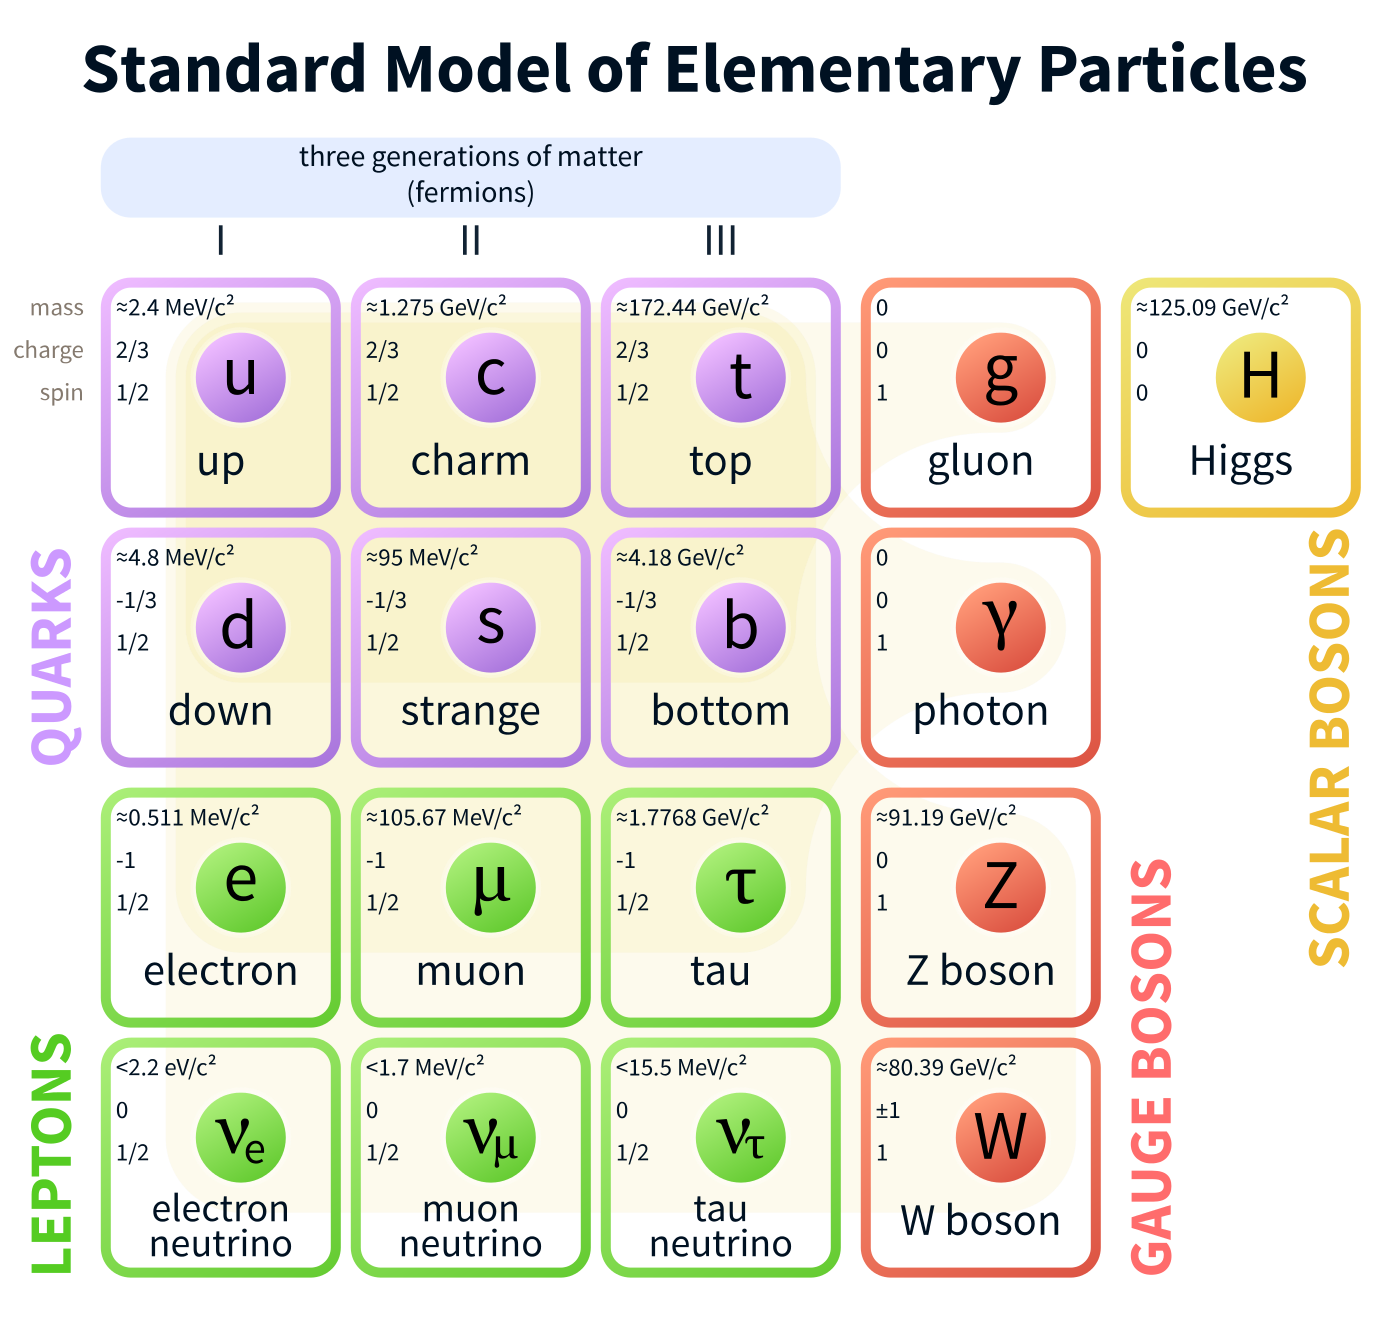
\includegraphics[width=0.6\textwidth]{Figures/Standard_Model_of_Elementary_Particles.png}
\caption[Standard Model]{The Standard Model describes all elementary particles, the twelve fermions in their three generations and the four gauge bosons, as well as the Higgs boson.
The shadows indicate possible interactions between the fermions and gauge bosons.~\cite{SM}}
\label{fig:SM}
\end{figure}

\paragraph{Fermions}
Fermions are particles with a spin quantum number of $s = 1/2$. 
The spin is the particle's rotation about its central axis, and has a direction and a specific amplitude.
The amplitude can be calculated as $\frac{h}{2\pi}\sqrt{s(s+1)}$, with $h$ being the Planck constant.~\cite[p. 121]{Griffiths}
All fermions have a specific set of quantum numbers, so that by giving the electric charge, the spin, and the flavor,  all fermions can be identified precisely.
Table~\ref{tab:Fermions} lists all Standard Model fermions with their quantum numbers.
\begin{table}
\caption[Quantum numbers of the Standard Model fermions]{Quantum numbers of the Standard Model fermions. The table lists the values for the electric charge $q$, and the spin $s$ for all fermions, as well as the lepton number $L$ of the leptons and the quark flavor of the quarks. Their respective antiparticles are highlighted by the shaded background.~\cite[cf. p. 49]{Griffiths}}
\label{tab:Fermions}
\centering
\begin{tabularx}{\textwidth}{c|c|rrrrr|@{\hskip 0.03in}|c|rrrrrrrr}
\hline\hline
& Leptons & $q$ & $s$ & $L_e$ & $L_{\mu}$ & $L_{\tau}$ & Quarks & $q$ & $s$ & $U$ & $D$ & $C$ & $S$ & $T$ & $B$\\
\hline
& e\textsuperscript{--} & --1 & 1/2 & +1 & 0 & 0 & u & +2/3 & 1/2 & +1 & 0 & 0 & 0 & 0 & 0\\
\rowcolor{Gray}
\cellcolor{white}& e\textsuperscript{+} & +1 & 1/2 & --1 & 0 & 0 & $\bar{\rm{u}}$ & --2/3 & 1/2 & --1 & 0 & 0 & 0 & 0 & 0\\
& $\upnu$\textsubscript{e} & 0 & 1/2 & +1 & 0 & 0 & d & --1/3 & 1/2 & 0 & --1 & 0 & 0 & 0 & 0\\
\rowcolor{Gray}
\multirow{-4}{*}{\rotatebox[origin=c]{90}{\parbox[c]{1.9cm}{\cellcolor{white}\centering First generation}}} &$\bar\upnu$\textsubscript{e} & 0 & 1/2 & --1 & 0 & 0 & $\bar{\rm{d}}$ & +1/3 & 1/2 & 0 & +1 & 0 & 0 & 0 & 0\\
\hline
& $\upmu$\textsuperscript{--} & --1 & 1/2 & 0 & +1 & 0 & c & +2/3 & 1/2 & 0 & 0 & +1 & 0 & 0 & 0\\
\rowcolor{Gray}
\cellcolor{white}&$\upmu$\textsuperscript{+} & +1 & 1/2 & 0 & --1 & 0 & $\bar{\rm{c}}$ & --2/3 & 1/2 & 0 & 0 & --1 & 0 & 0 & 0\\
& $\upnu$\textsubscript{$\upmu$} & 0 & 1/2 & 0 & +1 & 0 & s & --1/3 & 1/2 & 0 & 0 & 0 & --1 & 0 & 0\\
\rowcolor{Gray}
\multirow{-4}{*}{\rotatebox[origin=c]{90}{\parbox[c]{1.9cm}{\cellcolor{white}\centering Second generation}}}& $\bar\upnu$\textsubscript{$\upmu$} & 0 & 1/2 & 0 & --1 & 0  & $\bar{\rm{s}}$ & +1/3 & 1/2 & 0 & 0 & 0 & +1 & 0 & 0\\
\hline
& $\uptau$\textsuperscript{--} & --1 & 1/2 & 0 & 0 & +1 & t & +2/3 & 1/2 & 0 & 0 & 0 & 0 & +1 & 0\\
\rowcolor{Gray}
\cellcolor{white}& $\uptau$\textsuperscript{+} & +1 & 1/2 & 0 & 0 & --1 & $\bar{\rm{t}}$ & --2/3 & 1/2 & 0 & 0 & 0 & 0 & --1 & 0\\
& $\upnu$\textsubscript{$\uptau$} & 0 & 1/2 & 0 & 0 & +1 & b & --1/3 & 1/2 & 0 & 0 & 0 & 0 & 0 & --1\\
\rowcolor{Gray}
\multirow{-4}{*}{\rotatebox[origin=c]{90}{\parbox[c]{1.9cm}{\cellcolor{white}\centering Third generation}}}& $\bar\upnu$\textsubscript{$\uptau$} & 0 & 1/2 & 0 & 0 & --1 & $\bar{\rm{b}}$ & +1/3 & 1/2 & 0 & 0 & 0 & 0 & 0 & +1\\
\hline\hline
\end{tabularx}
\end{table}
Fermions are further categorized as \textit{leptons} and \textit{quarks}, as well as in three generations, which can be seen in Figure~\ref{fig:SM}.
Among the leptons, there are the electron and its heavier brothers, the muon and the tau.
In their respective generation, each of them has a neutrino, hence there are the electron-neutrino, muon-neutrino, and tau-neutrino, which are electrically neutral particles.\\
Since the SM does in general not remark the corresponding antiparticles, there are actually not only six leptons but twelve.
The only difference between particles and antiparticles is the sign of their internal quantum numbers:
The electron's antiparticle is the positron, which has the same mass and spin as the electron, but has a positive charge of +1, and a negative lepton number $L_e$ of -1.
The antiparticles of the muon ($\upmu$\textsuperscript{-}) and the tau ($\uptau$\textsuperscript{-}) hence are $\upmu$\textsuperscript{+} and $\uptau$\textsuperscript{+}, respectively.
As neutrinos on the other hand have no electric charge, they can only be distinguished from their respective antineutrino by their lepton number and their helicity.
The helicity describes the state of the particle's spin direction in comparison to the particle's momentum.
When the spin direction and the momentum are parallel, the particle is called right-handed.
It is called left-handed, when they are antiparallel.
In the SM, neutrinos are always left-handed, whilst antineutrinos are right-handed.
So far, no experiment has shown the opposite.\\
Every generation of quarks consists of one up- and one down-type quark, where the up-type quarks have an electric charge of 2/3, whilst down-type quarks have a charge of --1/3.
However, they do not only carry the electric charge, but also the so-called color charge.
Every quark has one of three colors (red, green, and blue), every antiquark has one of three anti-colors (anti-red, anti-green, and anti-blue).
Thus, there are overall 36 different quarks and antiquarks.
Due to the physics law of confinement, there can only be color-neutral particles.
Quarks are therefore not free, but hadronize and form a bound state together with other quarks.
These bound quark states, called hadrons, consist of either two, three, or five quarks.
A particle with a quark of a specific color and an antiquark of the corresponding anti-color is called a meson.
A baryon, which is a particle with three quarks, can only be color-neutral when it carries three quarks with three different colors (or anti-colors), so red--green--blue or anti-red--anti-green--anti-blue.
Any other combination is not possible.
Finally, the penta-quarks are bound states from five quarks, where three of them form a color triplet like a baryon, and the remaining two form a color-anticolor pair like a meson.\\
In everyday nature, the only observable hadrons are the protons and neutrons.
They are baryons, hence are built from three quarks:
protons contain two up-quarks and one down-quark, giving the proton its positive electric charge of +1.
Neutrons on the other hand are formed by one up-quark and two down-quarks, resulting in an electrically neutral particle. 
Together, they construct the nuclei of every atom of every element.
%The masses of the quarks increases towards higher generations.

\paragraph{Bosons}
Other than fermions, \textit{gauge bosons} are particles with a spin of +1.
The gauge bosons described in the SM are the force mediators of the fundamental forces of nature, except gravity.
The fermions explained above are subject to the fundamental forces, and can interact with each other by exchanging these gauge bosons.\\
The photon is a massless particle mediating the electromagnetic force.
Gluons are massless particles as well.
They carry the strong force, and are like the quarks also color-charged.
Therefore they cannot occur in isolation.
W and Z bosons on the other hand are massive particles, which are responsible for the weak force.\\
Gravity is the only fundamental force that is not represented by the SM.
On the scale of particle physics, it is by far the weakest force.

In contrast to the gauge bosons, the \textit{Higgs boson} has not got a spin of +1, but a spin of 0.
It is therefore a scalar boson.
The Higgs is the mediator of the Higgs field which is responsible for giving the mass to massive particles.

\todo{Explain deep inelastic scattering}

\section{Production modes}
\label{Production_modes}

\begin{figure}
\centering
\begin{subfigure}[b]{0.4\textwidth}
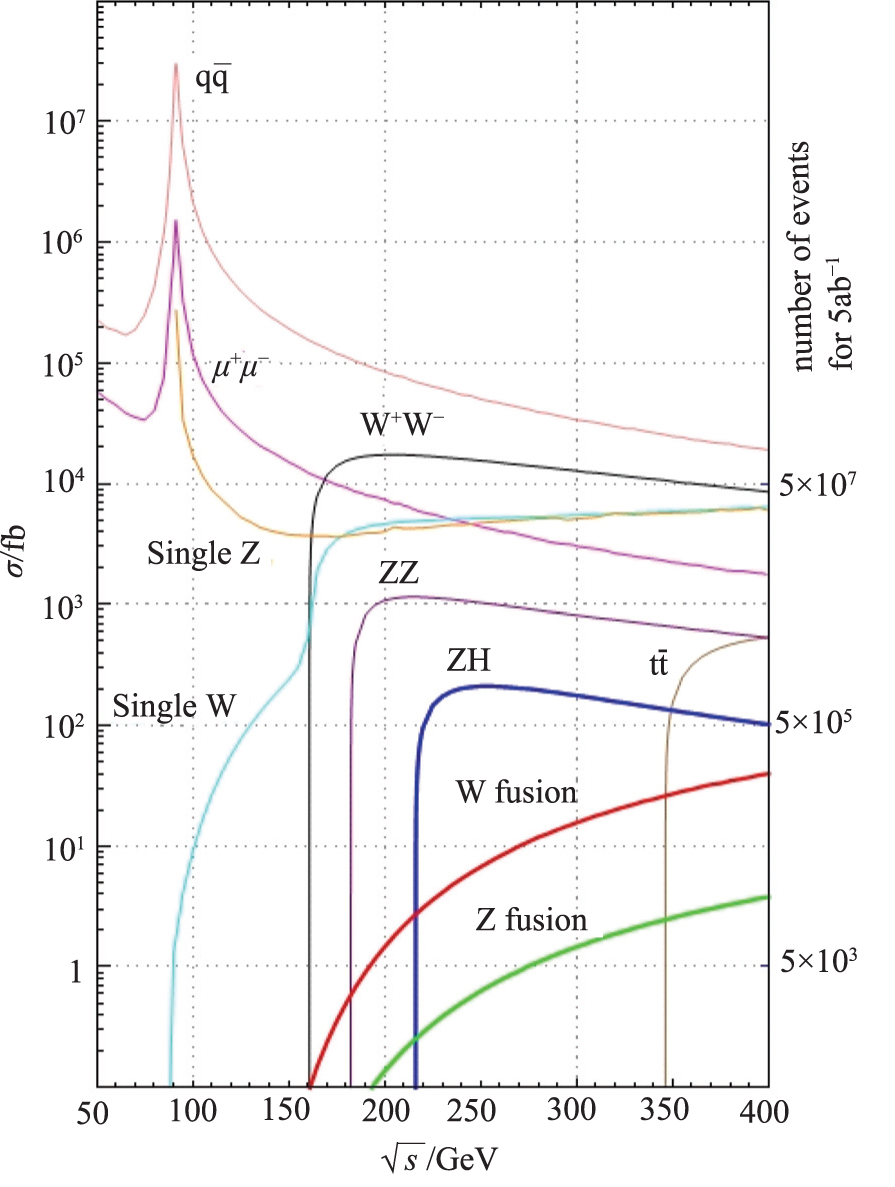
\includegraphics[width=0.98\textwidth]{Figures/ILC_cross_section.png}
\caption{\positron \electron cross-section~\cite{ILC_cross}}
\end{subfigure}
\begin{subfigure}[b]{0.4\textwidth}
\includegraphics[width=\textwidth]{Figures/LHC_cross_section.png}
\caption{pp cross-section~\cite{LHC_cross}}
\end{subfigure}
\caption[Cross sections for ILC and LHC]{Cross section at \positron \electron and pp colliders as a function of the collision energy. }%https://arxiv.org/pdf/hep-ph/0410364.pdf
\label{fig:Cross_sections}
\end{figure}

\section{Backgrounds}
\label{Backgrounds}
\subsection{High cross-section backgrounds from beam-beam interactions}
\label{BeamBeam}
\subsubsection{Pair background}
\label{BeamBeam:pairs}
\todo{Re-write this paragraph}
%Found here: http://www.sciencedirect.com/science/article/pii/S0168900216310919
For a Gaussian beam, the average energy $E_{\gamma}$ of photons from the deflection of the colliding particles is proportional to [5]:
\begin{equation}
 E_{\gamma} \propto \frac{N}{(\sigma_x+\sigma_y)\sigma_z}
 \label{eq:pair_energy}
\end{equation}
where N is the number of particles per bunch. The average number of photons is proportional to:
\begin{equation}
 n_{\gamma} \propto \frac{N}{(\sigma_x+\sigma_y)}
 \label{eq:pair_number}
\end{equation}
%Therefore, in ILC chapter about beam parameters: Hence flat beams with $\sigma_x\gg\sigma_y$ are used. The product of the horizontal and vertical beam sizes is small leading to high luminosity while the sum of them is large, reducing the beamstrahlung effect.

\begin{figure}
\begin{subfigure}[b]{0.33\textwidth}
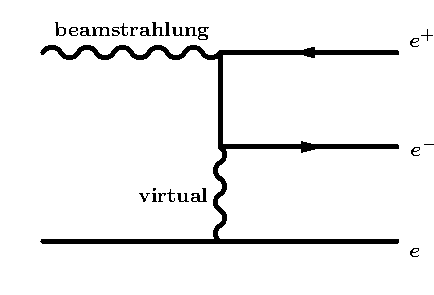
\includegraphics[width=\textwidth]{Figures/Bethe-Heitler.pdf}
\caption{Bethe-Heitler}
\end{subfigure}
\begin{subfigure}[b]{0.33\textwidth}
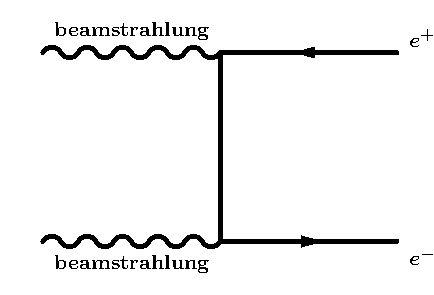
\includegraphics[width=\textwidth]{Figures/Breit-Wheeler.pdf}
\caption{Breit-Wheeler}
\end{subfigure}
\begin{subfigure}[b]{0.33\textwidth}
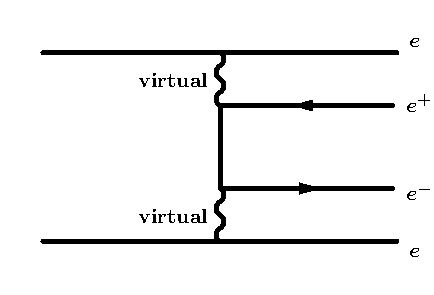
\includegraphics[width=\textwidth]{Figures/Landau-Lifshitz.pdf}
\caption{Landau-Lifschitz}
\end{subfigure}
\caption[LO Feynman diagrams of the production of the background pairs.]{The LO Feynman diagrams of the production processes of the background pairs: Bethe-Heitler, Breit-Wheeler and Landau-Lifschitz.}
\label{fig:Feynman:pair_production}
\end{figure}

\subsubsection{Bhabha scattering and $\gamma\gamma\rightarrow$hadrons}
\label{BeamBeam:bhabha_gammagamma}

\begin{figure}
\centering
\begin{subfigure}[b]{0.35\textwidth}
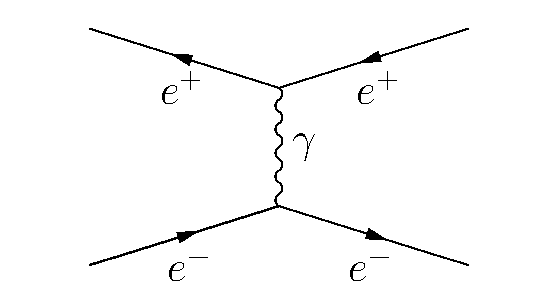
\includegraphics[width=\textwidth]{Figures/bhabha_scattering.pdf}
\caption{Bhabha scattering}
\end{subfigure}
\vspace*{0.2cm}
\begin{subfigure}[b]{0.35\textwidth}
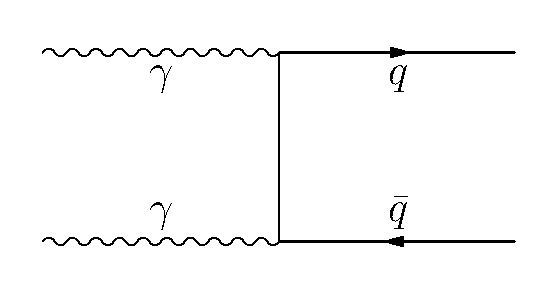
\includegraphics[width=\textwidth]{Figures/gammagamma_hadrons.pdf}
\caption{$\gamma\gamma\rightarrow$hadrons}
\end{subfigure}
\caption[LO Feynman diagrams of bhabha scattering and the $\gamma\gamma\rightarrow$hadrons process.]{The LO Feynman diagrams of the bhabha scattering and the $\gamma\gamma\rightarrow$hadrons process.}
\label{fig:Feynman:bhabha_gammagamma}
\end{figure}

\subsection{Machine backgrounds}
\label{MachineBackgrounds}